\documentclass[varwidth,convert={density=500,size=1080x800,outext=.png}]{standalone}
\usepackage{tikz}
\usetikzlibrary{calc,patterns,decorations.pathmorphing,decorations.markings}
\usepackage{pgfplots}
\usepackage{stanli}

\usepackage[dvipsnames]{xcolor}

\begin{document}
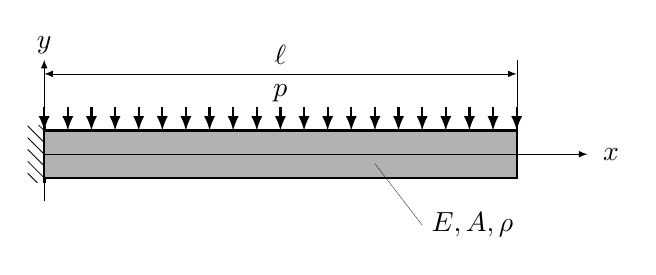
\begin{tikzpicture}[scale=0.6]
        \point{a}{0}{0.3};
        \support {3}{a}[270];
        % Draw the rectangle
        \filldraw[fill=gray!60, draw=black,thick] (0,0) rectangle (10,1);
        %axis
        \draw[-latex, ultra thin] (0,0.5) -- (11.5,0.5);
        \draw[-latex, ultra thin] (0,-0.5) -- (0,2.5);
        \node at (12,0.5) {\(x\)};
        \node at (0,2.8) {\(y\)};
        % length
        \draw[ultra thin] (10,0) -- (10, 2.5) ;
        \draw[latex-latex, ultra thin]  (0,2.2)  to node[sloped,midway,above] {$\ell$}(10,2.2) ;
        % M and V 
         \foreach \i in {0,...,20}
          {
            \draw[-latex, thick]  (0.5*\i,1.5)--(0.5*\i,1);
          }
                  \node at (5,1.8) {\(p\)};

        \draw[ultra thin]  (7,0.3) -- (8,-1) node[right]{$E,A,\rho$};
      \end{tikzpicture}


\end{document}